%
% LaTeX template for prepartion of submissions to PLDI'15
%
% Requires sigplanconf style file provided on PLDI'15 web site
%
\documentclass[pldi,blind,clearpagebib]{sigplanconf-pldi15}

%
% the following standard packages may be helpful, but are not required
%
\usepackage{SIunits}            % typset units correctly
\usepackage{courier}            % standard fixed width font
\usepackage[scaled]{helvet} % see www.ctan.org/get/macros/latex/required/psnfss/psnfss2e.pdf
\usepackage{url}                  % format URLs
\usepackage{listings}          % format code
\usepackage{fancyvrb}
\usepackage{graphicx}
\usepackage{subfig}
\usepackage{enumitem}      % adjust spacing in enums
\usepackage[colorlinks=true,allcolors=blue,breaklinks,draft=false]{hyperref}   % hyperlinks, including DOIs and URLs in bibliography
% known bug: http://tex.stackexchange.com/questions/1522/pdfendlink-ended-up-in-different-nesting-level-than-pdfstartlink
\newcommand{\doi}[1]{doi:~\href{http://dx.doi.org/#1}{\Hurl{#1}}}   % print a hyperlinked DOI



\begin{document}

%
% any author declaration will be ignored  when using 'plid' option (for double blind review)
%

\title{Declarative coordination of parallel declarative programs}
\authorinfo{Flavio Cruz}
           {Carnegie Mellon University\\Pittsburgh, PA 15213, USA}
           {fmfernan@cs.cmu.edu}

\authorinfo{Ricardo Rocha}
           {CRACS \& INESC TEC\\University of Porto\\Rua Campo Alegre 1021/1055\\4169-007 Porto, Portugal}
           {ricroc@dcc.fc.up.pt}

\authorinfo{Seth Copen Goldstein}
           {Carnegie Mellon University\\Pittsburgh, PA 15213, USA}
           {seth@cs.cmu.edu}

\maketitle
\begin{abstract}
Declarative programming has been hailed as a promising approach to parallel
programming since it hides the implementation details of parallelism away from the
programmer. However, its advantage has also been its downfall
as it leaves the programmer with no straightforward way
to optimize programs for performance.
In this paper, we introduce Coordinated Linear Meld, a concurrent forward-chaining linear logic programming
language, with a declarative way to coordinate the execution of the program
allowing the programmer to change
computation scheduling and data layout. Our approach allows the programmer to
write declarative parallel programs and then optionally use coordination 
to fine tune programs, while keeping the program fully declarative and easy to
reason about.

\end{abstract}

\category{D.1.3}{PROGRAMMING TECHNIQUES}{Concurrent Programming}[Parallel Programming]
\category{D.3.4}{PROCESSORS}{Interpreters}
\category{D.3.4}{PROCESSORS}{Run-time environments}

\terms{Design, Languages, Performance}

\keywords{Parallel Programming, Linear Logic, Virtual Machine, Implementation}

\section{Introduction}
Parallel programming in sequential languages is hard because manipulating a
shared state using multiple threads may result in data race conditions. Such
issues are handled with low level constructs such as locks, semaphores and/or condition
variables, requiring a fair amount of effort to get right.  Declarative
programming has been hailed as a alternative solution to this issue, since the problem of
implementing the details of parallelism is moved from the programmer to the
compiler and runtime environment. The programmer writes code without having to deal with
parallel programming constructs and the compiler automatically parallelizes the
program in order to take advantage of multiple threads of execution.  This
programming paradigm has been adopted with huge success in domain specific
languages such as SQL and MapReduce~\cite{Dean:2008:MSD:1327452.1327492}.
Although general declarative languages have yet to be as successful, the future
looks promising for this particular approach.

The problem with declarative programming is that it leaves little to no
programmer control over how execution is scheduled or how data is laid out,
making it hard to improve efficiency. This introduces
performance issues because even if the runtime system is able to
reasonably parallelize the program using a general algorithm, there
is a lack of specific information about the program that a compiler
cannot easily deduce. Such information could make execution better in
terms of run time time, memory usage, and/or scalability.

In this paper, we introduce Coordinated Linear Meld (CLM), a data-centric declarative
language that extends the Linear Meld~(LM)
language~\cite{cruz-iclp14,cruz-ppdp14} with coordination facts that give
programmer control over scheduling and data placement. LM is a linear logic
programming language designed for programs that operate on graphs.  The use
of linear logic~\cite{girard-87} supports structured manipulation of mutable
state. In LM, computation is divided so that each node of the graph computes
independently but is allowed to \scare{communicate} with other nodes.  Both
computation and communication happen through the derivation of logical rules
(which make up the program).

The CLM language features two kinds of coordination primitives that can be used in the same
way as any other primitive, i.e., they are specified with the same
syntax and semantics as the rest of the programming language. These coordination
primitives can be used to improve program execution based on the state of the
program and the underlying machine. The first kind of coordination primitives are
called \emph{sensing facts} and are used to sense information about the system
the program is running on, e.g., scheduling and node placement on threads. The
second kind of coordination primitives are \emph{action facts} that when detected in
rules, are used to apply a scheduling operation during execution. Coordination
facts allow the programmer to write logical rules that depend on the current
state of the program and then prioritize node computation or place nodes in
different threads.

To the best of our knowledge, this is the first time that a declarative language
allows control over execution while staying declarative and without resorting to
meta-language constructs. This is crucial to our goal of being able to prove
programs correct since proofs can be constructed even in the presence of
coordination facts.  After briefly discussing related work, we present an
overview of the base language, with an example. In
\sectref{sec:coordination}, we introduce the current set of coordination
facts, followed by a description of the changes required to implement the
desired coordination mechanisms. In \sectref{sec:applications} we present
several applications and show how coordination can improve programs without
destroying clarity or provability.


\section{Related Work}
Recently, there has been an increasing interest in declarative and data-centric
languages. MapReduce~\cite{Dean:2008:MSD:1327452.1327492}, for instance, is a
popular data-centric programming model that is optimized for large clusters. The
scheduling and data sharing model is very simple: in the \emph{map phase}, data
is transformed at each node and the result reduced to a final result in the
\emph{reduce phase}. Like LM, many programming systems model the program as a
graph where computation will be performed. The Dryad
system~\cite{Isard:2007:DDD:1272996.1273005} combines computational vertices
with communication channels (edges) to form a data-flow graph. The program is
scheduled to run on multiple computers or cores and data is partitioned
automatically during runtime.

Many programming languages follow the so-called \emph{coordination
paradigm}~\cite{Papadopoulos98coordinationmodels}, a form of distributed
programming that divides execution in two parts: \emph{computation}, where the actual
computation is performed, and \emph{coordination}, which deals with
communication and cooperation between processing units. This paradigm attempts
to clearly distinguish between these two parts by providing abstractions for
coordination in an attempt to provide architecture and system-independent forms
of communication.  

Linda~\cite{linda} is probably the most famous coordination model. Linda
implements a data-driven coordination model and features a \emph{tuple space}
that can be manipulated using the following coordination directives:
\texttt{out(t)} writes a tuple \texttt{t} into the tuple space; \texttt{in(t)}
reads a tuple using the template \texttt{t}; \texttt{rd(t)} retrieves a copy of
the tuple \texttt{t} from the tuple space; and \texttt{eval(p)} puts a process
\texttt{p} in the tuple space and executes it in parallel. 
Linda is be implemented on top of many
popular languages by simply creating a communication and storage mechanism for
the tuple space and then adding the directives as a language library.

Another coordination language is Delirium~\cite{Delirium}, where instead of being
embbeded in another language like Linda, it actually embeds operators other
languages inside Delirium. The advantages of Delirium are improved abstraction
and easier debugging because sequential operators are isolated from the
coordination language.

Linda and Delirium are limited in the sense that the programmer can only
coordinate the scheduling of processing units, while the placement of data is
left to the implementation. LM also differs from those languages since it
raises the abstraction level from the processing units to nodes of a graph,
which are part of the program logic.
Furthermore, the language LM is both the coordination and the computation
language and there is no distinction between them.

\iffalse
GraphLab~\cite{GraphLab2010} is a C++ framework for developing parallel machine
learning algorithms. GraphLab allows nodes to
have read/write access to different scopes through different concurrent access
models in order to balance performance and data consistency. While some programs
only need to access the local node's data, others may need to update edge
information. Each consistency model will provide different guarantees that are
better adapted to some algorithms. GraphLab provides different schedulers
that dictate the order in which node's are computed, which is a rudimentary form
of coordination. Later in this paper, we will show how certain GraphLab's
schedulers can be easily implemented in LM through the use of coordination
facts.
\fi


\section{Base Language}\label{sec:language}

Linear Meld (LM) is a forward-chaining linear logic programming
language~\cite{cruz-iclp14} with roots on Datalog~\cite{Ramakrishnan93asurvey}.
Programs are written as a set of rules of the form
\texttt{a(X), b(Y) -o c(Z)} and are read as following: if \texttt{a(X), b(Y)} (the body of
the rule) is satisfied using some facts \texttt{a(X)} and \texttt{b(Y)} then
\texttt{c(Z)} (the head of the rule) is true.
The facts used during rule derivation are placed in a \emph{database of facts}.
Logical facts are composed of a predicate and a tuple of concrete values,
representing the arguments.
Since LM uses linear logic as its foundation, rule derivations
may delete facts used in the body of the rule. Program execution starts by
adding the \emph{axioms} (the initial facts) of the program to the database.
Next, the rules are recursively applied and the database is updated with new and
deleted facts. When nore more rules are applicable, the program terminates.

LM has been designed for writing graph-based programs. LM accomplishes this by
partitioning the logical facts by the first argument (the \emph{node}) and by
restricting the body of every rule to only refer to the same first argument.
This allows rules to be executed using only facts of a single node. Although the
body of rules is restricted, the head of the rule may refer to any other node as
long as the node variable is refered somewhere in the body of the rule. This allows
derivations of facts in other nodes. The whole database is then composed of smaller
databases (the nodes) and rule derivations allows smaller databases to derive
facts in other databases, creating edges in the graph.

In order to fully understand how the language works, we present a very simple
algorithm: the single source shortest path program~(SSSP). Later in the paper, we
add coordination facts to improve the execution of the program.

The SSSP program in Fig.~\ref{code:shortest_path_program} starts (lines 1-3)
with the declaration of the predicates. Predicates specify the kinds of facts
used in the program. The first predicate, \texttt{edge}, specifies edges between
nodes of the graph, where the third argument represents the weight of the edge.
The \texttt{route} modifier informs the compiler about the structure of the
program graph. The predicates \texttt{shortest} and \texttt{relax} are specified
as linear facts and thus are deleted when used in rules.
The idea of the algorithm is to compute the shortest distance from node
\texttt{@1} to all other nodes in the graph. Every node has a \texttt{shortest}
fact that is improved with new \texttt{relax} facts.
Lines 5-9 declare the axioms of the program: \texttt{edge} facts describe the
graph; \texttt{shortest(A, +00, [])} is the initial shortest distance (infinity)
for all nodes; and \texttt{relax(@1, 0, [@1])} starts the algorithm with the
initial distance from \texttt{@1} to \texttt{@1}.

\begin{figure}[h!]
\scriptsize\begin{Verbatim}[numbers=left]
type route edge(node, node, int).
type linear shortest(node, int, list int).
type linear relax(node, int, list int).

!edge(@1, @2, 3). !edge(@1, @3, 1).
!edge(@3, @2, 1). !edge(@3, @4, 5).
!edge(@2, @4, 1).
shortest(A, +00, []).
relax(@1, 0, [@1]).

relax(A, D1, P1), shortest(A, D2, P2),
D1 < D2
   -o shortest(A, D1, P1),
      {B, W | !edge(A, B, W) |
         relax(B, D1 + W, P1 ++ [B])}.

relax(A, D1, P1), shortest(A, D2, P2),
D1 >= D2
   -o path(A, D2, P2).
\end{Verbatim}
  \caption{Single Source Shortest Path program code.}
  \label{code:shortest_path_program}
\end{figure}
\normalsize

The first rule of the program (lines 11-15) replaces the current path in
\texttt{shortest} with a shorter one in \texttt{relax}. The rule deletes both
\texttt{relax} and \texttt{shortest} facts and derives a new \texttt{shortest}
fact. In lines 14-15, we have a \emph{comprehension} where the program iterates
over the edges of node \texttt{A} and derives a new \texttt{relax} fact at
\texttt{B} with the new shorter distance plus the weight of the edge. For
instance, in Fig.~\ref{fig:shortest_path_program}~(a) we apply rule 1 in node
\texttt{@1} where two new \texttt{relax} facts are derived at node \texttt{@2}
and \texttt{@3}. Fig.~\ref{fig:shortest_path_program}~(b) is the result after
applying the same rule but at node \texttt{2}.

\begin{figure*}[ht]
\begin{center}
  \subfloat[]{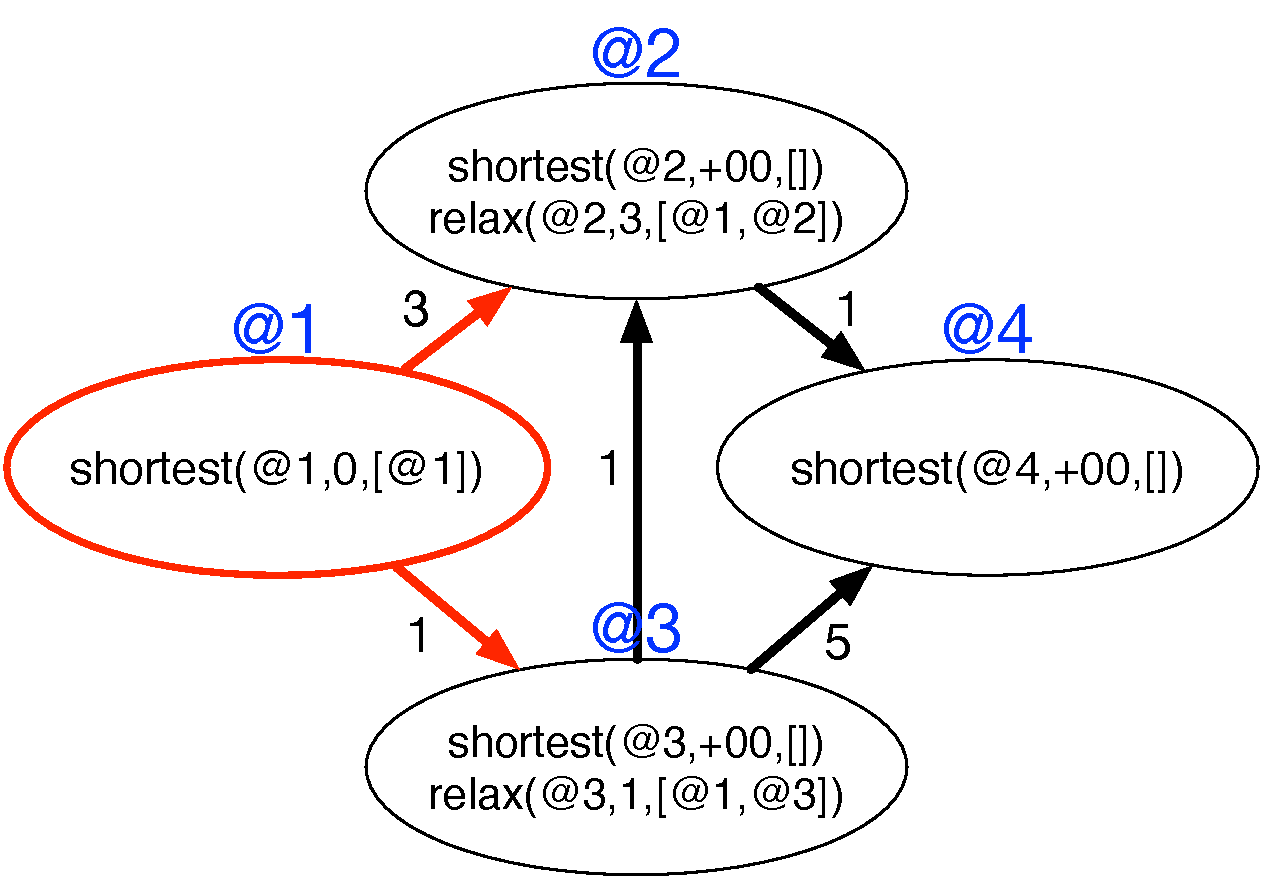
\includegraphics[width=0.3\textwidth]{figures/shortest2}}
  \subfloat[]{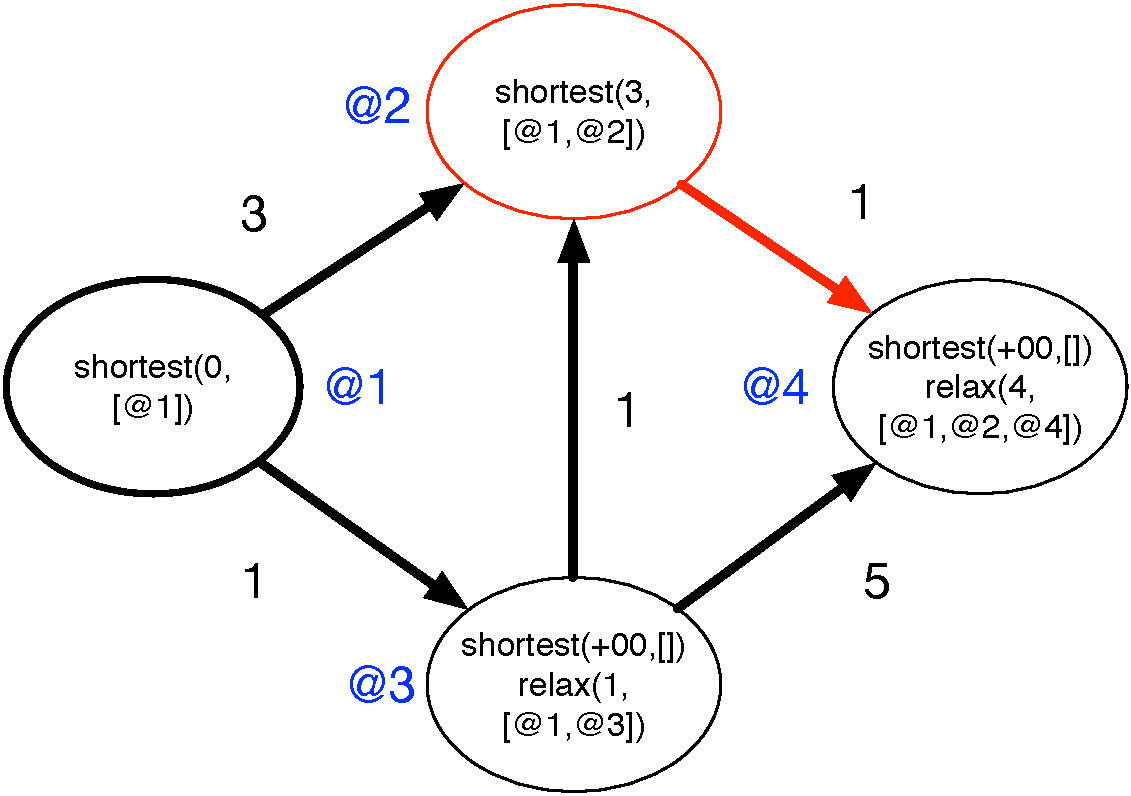
\includegraphics[width=0.3\textwidth]{figures/shortest3}}
  \subfloat[]{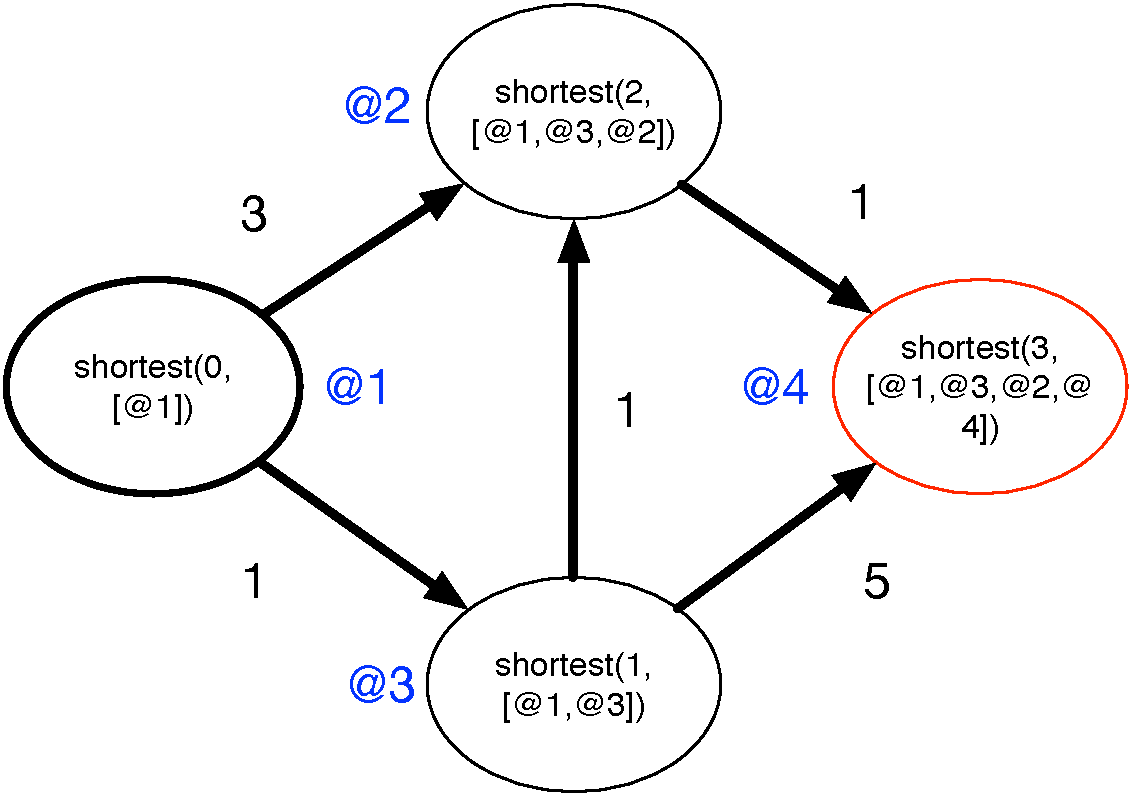
\includegraphics[width=0.3\textwidth]{figures/shortest8}}
\end{center}
\caption{Graphical representation of the SSSP program. Figure (a) represents the
   program after propagating initial distance at node \texttt{@1}, followed by
   Figure (b) where the first rule is applied in node \texttt{@3}. Figure (c)
   represents the state of the final program, where all the shortest paths
   have been computed.}
\label{fig:shortest_path_program}
\end{figure*}

The second rule of the program (lines 17-19) deals with the case where the new
distance in \texttt{relax} is not better than the current one, so it is thrown
away and the current distance is kept.

There many opportunities for concurrency in the SSSP program. For instance,
after applying rule 1 in Fig.~\ref{fig:shortest_path_program}~(a), it is
possible to either apply rules in either node \texttt{@2} or node
\texttt{@3}. In our implementation, we partition the graph into subgraphs that
are processed by multiple threads of execution. Eventually, it is no longer to
possible to apply rules and the final result present in
Fig.~\ref{fig:shortest_path_program}~(c) is achieved.

%On the other hand, LM has no natural matching of data and computation to workers (processes, threads),
%since nodes are a program abstraction and part of the program's logic.
%We view the set of nodes as a graph data structure where workers will perform work.
%A worker is able to process any node, although a node cannot be computed by more than one worker
%at the same time. This disallows the manipulation of a node by multiple workers.



\section{Coordination}\label{sec:coordination}
Since LM uses linear logic and supports deletion of facts, the order in which
nodes are scheduled can impact the performance and even the results of the
program.

The SSSP program present in Fig.~\ref{code:shortest_path_program} is concise and
declarative but its performance may depend in the order in which nodes are
executed. If nodes with greater distances are prioritized over other nodes, the
program will generate more \texttt{relax} facts since it will take longer to
reach the shortest distances. From Fig.~\ref{fig:shortest_path_program}, it is
clear that the best computational ordering is the following: \texttt{@1},
\texttt{@3}, \texttt{@2} and then \texttt{@4}, where only 4 \texttt{relax}
facts are generated. If we had decided to process nodes in order
\texttt{@1}, \texttt{@2}, \texttt{@4}, \texttt{@3}, \texttt{@4},
\texttt{@2}, then 6 \texttt{relax} facts would have been generated.
Therefore, the optimal solution for SSSP is to schedule the node with the
shortest distance, which is essentially the Dijkstra shortest path
algorithm~\cite{Dijkstra}. Note how it is possible to change the nature of
the algorithm by simply changing the order of node computation, but still
retain the declarative nature of the program.

We introduce the concept of \emph{coordination facts} that allow the programmer
to change how the run time schedules nodes and partitions the nodes among
threads of execution. Coordination facts can be used in the body or head of the
rules to allow the programmer to reason and change how execution is to be done.
In this fashion, we keep the language declarative because we reason logically
about the state of execution, without the need to introduce extra-logical
operators into the language that would introduce problems when attempting to prove
properties about programs.

There are two classes of coordination facts. The first class of coordination facts are
called \emph{sensing facts} and are used to sense information about the
underlying runtime system, including node placement and node scheduling.
The second kind of coordination facts are \emph{action facts} that are deleted
to apply a coordination operation in the runtime system.

\subsection{Scheduling Facts}\label{sec:fifo}

We can use action facts to change the order in which nodes are evaluated by adding
\emph{priorities}. Node priority works at the thread level
so that each thread can make a local decision about which node to execute next.
Note that, by default, nodes are picked using a FIFO approach, because that
tends to work better for most programs since older nodes tend to have more facts
to be used.

We have two kinds of priorities: a \emph{temporary priority} and a \emph{default
priority}. A temporary priority momentarily changes the default priority $D$ of a
node, so that once the node is done, the priority will default back to $D$.
Initially, all nodes have a default priority of $0$.

The following list presents the action facts available to manipulate the scheduling
decisions of the system:

\begin{itemize}
   \item \texttt{type linear set-priority(node, float)}: This sets the
   temporary priority of a node. If the node already has a priority, we only
   change the priority if the new one is higher. The programmer can
   decide if priorities are to be ordered in ascending or descending order.
   \item \texttt{type linear action add-priority(node, float)}: Increases,
   temporarily, the priority of the node.
   \item\texttt{type linear schedule-next(node)}: The work will fetch the
   highest priority node's priority $P$ from its set of nodes and set the
   action's argument node's priority as $P + 1.0$. If using the priorities in
   ascending order, we pick the lowest priority and subtract $1.0$.
   \item\texttt{type linear set-default-priority(node, float)}: Sets the default
   priority of the node.
   \item \texttt{type linear action stop-program(node)}: Immediately stops the
   execution of the whole program.
\end{itemize}

LM provides the sensing fact \texttt{priority(A, B, P)} in order to sense the
priority \texttt{P} of node \texttt{B} from node \texttt{A}.
Sensing facts are only used in the body of the rules in order
to fetch information from the runtime system.
Note that when sensing facts are deleted, they are re-derived automatically.
Logically, \texttt{set-priority} and \texttt{set-default-priority} update the
value of \texttt{priority} facts, but this done automatically by the runtime
system.

\subsubsection{Partitioning facts}

We provide several coordination facts for dealing with node partitioning among
the available threads executing the program. In terms of action
facts, we have the following:

\begin{itemize}
   \item \texttt{type linear set-cpu(node, int)}: Moves the node to a
   thread of execution.
   \item \texttt{type linear set-affinity(node, node)}: Places the first node in
   the same thread as the second node.
   \item \texttt{type linear set-moving(node)}: Allows the node to move freely
   between threads.
   \item \texttt{type linear set-static(node)}: Forces the node to stay in the
   same thread indefinitely.
\end{itemize}

For sensing facts, we have the following set of coordination facts:

\begin{itemize}
   \item \texttt{type linear cpu-id(node, node, int)}: The third argument
   indicates the thread where the node of the second argument is currently running.
   \item \texttt{type linear moving(node, node)}: Fact available if the node in the
   second argument is allowed to move between threads.
   \item \texttt{type linear static(node, node)}: Fact available if the node in
   the second argument is not allowed to move between threads.
\end{itemize}

\iffalse
\subsubsection{Global Directives}

We also provide a few global coordination statements:

\begin{description}
   \item[\texttt{priority @order ORDER.}] \texttt{ORDER} can be either \texttt{asc} or \texttt{desc}. This defines if node's are to be selected by the smallest or the greatest priority, respectively.
   \item[\texttt{priority @initial P.}] The \texttt{initial} statement informs the runtime system that all nodes must start with priority $P$. Alternatively, the programmer can define an \texttt{set-priority(A, P)} axiom.
   \item[\texttt{priority @static.}] The \texttt{static} priority tells the runtime system that the partition of nodes among workers is to be used until the end of program. 
\end{description}

\fi


\section{Implementation}\label{sec:implementation}
The implementation of LM includes a compiler and a virtual machine that runs
byte-code. The virtual machine uses 32 registers for
operations and executes procedures to iterate over the database in order to match facts.

\subsection{Compilation}

The compiler translates each rule to a procedure and a list of facts that need
to exist to satisfy the rule. This procedure is executed by the virtual
machine whenever we have enough facts to satisfy the rule. The procedure
loops over all possible combinations of the rule, retrieving facts from the
database, performing join operations and then consuming and deriving facts.

Optimizations such as join optimizations (to allow rule filtering invalid
combinations) and fact updates are implemented by the compiler. The latter
transforms fact derivations of the same predicate to a simple update operation,
avoiding a deallocation operation followed by an allocation of the new fact.

\subsection{Node partitioning}

The compiler builds a representation of the graph by inspecting axioms of the
program. Next, it orders the nodes of the graph using a breadth-first
topological sort. This node ordering is written to the byte-code file and then
used to initially partition nodes across available threads.

\subsubsection{Coordination directives}

Coordination directives are compiled in two different ways, depending whether they
appear in the body or in the head of the rule. Coordination facts in the body
are compiled into special instructions that inspect the state of the virtual
machine. For example, the directive \texttt{node-priority} will inspect the
target node, retrieve the current priority and assign the priority to a
register. Coordination facts in the head of the rule are also implemented as
special instructions of the virtual machine, but they perform some action,
instead of returning something. While these are still facts from the point of
view of the language, they are consumed immediatelly in order to apply the
operation, instead of being derived like any other regular fact. This is more
efficient since we do not need to create a new fact.

\subsection{Execution}

The virtual machine is implemented in C++11 and uses the threading system from
the standard library to implement multithreading. Each thread is responsible
for executing a subset of nodes. Nodes are either inactive, with no new facts,
or active, where they will be placed in the corresponding thread's queue.
Threads do useful work by processing the nodes in their queues. Whenever a
thread becomes idle, it attempts to steal nodes from a random thread into its
own queues. If unsuccessful, the thread synchronizes with the other threads to
become inactive.

\subsubsection{Nodes}

A node is represented as a collection of facts (per predicate) and an indexing structure that
keeps track of the available predicates and potential candidate rules. We need
a separate indexing structure per node since rules run locally.

Facts need to be stored efficiently because the virtual machine instructions
perform searches on the database by fixing arguments of a predicate to concrete
values. Each predicate is stored using one of the following data structures:

\begin{itemize}
\item \emph{Tries} are used exclusively to store 
  persistent facts. Tries are trees where facts are indexed by common
  prefix arguments.
\item \emph{Doubly Linked Lists} are used to store 
  linear facts. We use a double linked list because it is a very
   efficient way to add and remove facts.
\item \emph{Hash Tables} are used to improve lookup when 
  linked lists are too long and when we need to do search filtered by
  a fixed argument. The virtual machine decides which arguments are
  best to be indexed and then uses a hash table
  indexed by the appropriate argument.
\end{itemize}

A node goes through different states during execution. The state machine in
Fig.~\ref{fig:node_states} represents the valid state transitions with the
following states:

\begin{description}
   \item[working]: the node is being executed.
   \item[idle]: the node is not active, has no new facts and is not in any
   queue for processing.
   \item[queue]: the node is active with new facts and is waiting in some queue
   to be processed.
   \item[stealing]: the node has just been stolen is about to move to another
   thread.
   \item[coordinating]: the node is moving from one queue to another (i.e.
         changing priority).
\end{description}

\begin{figure}[h!]
   \centering
   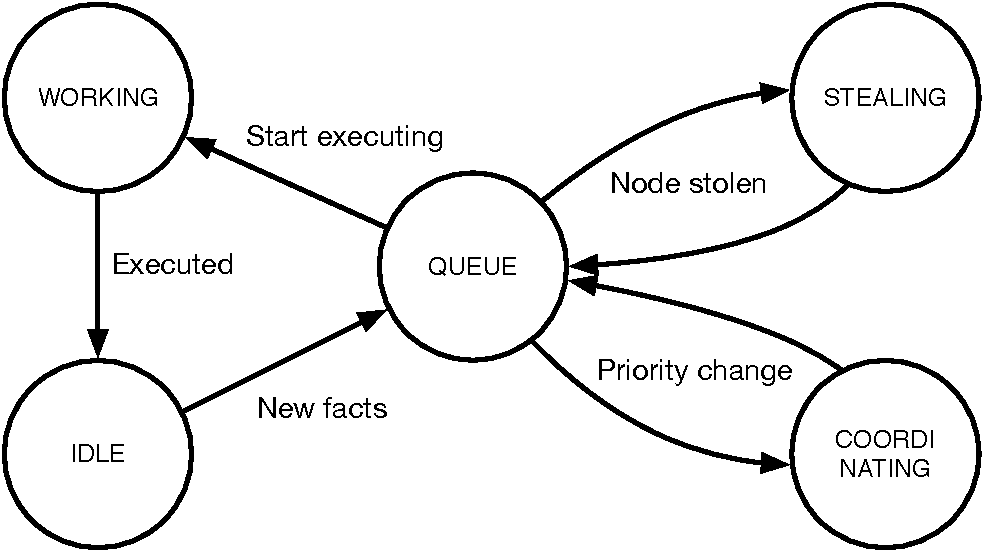
\includegraphics[width=0.4\textwidth]{node_states.pdf}
   \caption{The node state machine. During the lifetime of a program, each node
   goes through different states as specified by the state machine.}
   \label{fig:node_states}
\end{figure}

Each node is protected by a main spinlock that allows threads to change node
attributes: incoming facts, owner thread, node state and locality information.
There is also an internal spinlock that is locked whenever the node enters into
the \textbf{working} state. If a thread sends facts to a node placed in
another thread, it attempts to lock the internal lock in order to update the
indexing structures of the node, otherwise it adds the facts to the list of
incoming facts that are later processed by the owner thread.

\subsubsection{Threads}

Threads pop active nodes from their queues and execute new candidate rules. 
Each thread has 2 queues, a doubly linked list known as the \emph{standard
queue} and a min/max heap known as the \emph{priority queue}. The regular queue
contains nodes without priorities and
implements the operations \texttt{push\_tail(node)} (push to the tail),
\texttt{pop\_head()} (remove node from the head),
\texttt{remove(node)} (remove an arbitrary node) and \texttt{remove\_half()}
(removes first half). The priority queue contains nodes
with priorities and is implemented as a binary heap array. It supports the
operations \texttt{push(node,priority)} (add new node to the heap),
           \texttt{pop\_min()} (remove the best node),
\texttt{remove(node)} (remove an arbitrary node), \texttt{pop\_half\_min()}
(remove the best half) and \texttt{move(node,new\_priority)} (update priority).
Operations such as \texttt{remove\_half()} are supported in order to support
node stealing, while operations \texttt{remove(node)} or
\texttt{move(node,new\_priority)} allows threads to change the priority of
nodes.

The \texttt{next} and \texttt{prev} pointers of the regular queue are part of
the node structure in order to save space. These pointers are also used as the
index in the priority queue and current priority, respectively.

Both the regular and priority queue are actually implemented as 2 queues each.
The \emph{static queue} contains nodes that are local to a thread (and thus cannot be stolen) and
the \emph{dynamic queue} maybe accessed by other threads during node stealing.

\subsubsection{Communication}

Threads synchronize with each other using mutual exclusion. We use a spinlock in
each queue to protect queue operations and one spinlock to protect the thread's
state. Given threads $T_1$ and $T_2$, we enumerate the most important
synchronization intensive places in the virtual machine:

\begin{description}
   \item[New facts:] When a node executes on $T_1$ and derives facts
   to a node in $T_2$, $T_1$ first buffers the facts 
   and then sends them to the target node. Here, it checks if the
   node is currently \textbf{idle} and then synchronizes with $T_2$ to add the
   node to the $T_2$'s queue.
   \item[Thread activation:] If $T_2$ is inactive when adding facts to a node in
   $T_2$, $T_1$ also synchronizes with $T_2$ to change $T_2$'s state to \emph{active}.
   \item[Node stealing:] $T_1$ synchronizes with $T_2$ when it attempts to steal
   nodes from $T_2$ by removing half of the nodes from $T_2$'s queues.
   \item[Coordination:] If $T_1$ needs to perform coordination operations
   to a node in $T_2$, it may need to sychronize with $T_2$ during priority
   updates in order to move the node in $T_2$'s queues.
\end{description}

\subsubsection{Termination}

There is a global atomic counter, a global boolean flag and one boolean flag
(active/idle) per thread for detecting termination. Once a thread goes idle,
it decrements the global counter and changes its flag to idle. If the counter
goes to zero, the global flag is set to idle. Since every thread will be
busy-waiting and checking the global flag, they will detect the change and exit
the program.



\section{Applications}\label{sec:applications}

To better understand how coordination facts are used, we next present some programs that
take advantage of them. In our experimental setup, we we used a machine with
four AMD Six-Core Opteron TM 8425 HE (2100 MHz) chips (24 cores) and 64 GB of
DDR-2 667MHz (16x4GB) RAM, running GNU/Linux (kernel 3.15.10-201 64 bits).
We compiled our virtual machine using GCC 4.8.3 (g++) with the flags
\texttt{-O3 -std=c++11 -fno-rtti -march=x86-64}~\footnote{Implementation
   available in \url{http://github.com/.../meld}}.

\subsection{Single Source Shortest Path}
Here we add coordination to the SSSP program described in \sectref{sect:ssspex}.
The coordinated version of the
SSSP~(Fig.~\ref{code:shortest_path_program_coord}) uses the coordination fact
\texttt{set-priority} (line 14). We also use a global program directive to order
priorities in ascending order (line 5).

When run with one thread, the algorithm behaves like
Dijkstra's shortest path algorithm~\cite{Dijkstra}. When using multiple
threads, each thread will pick the smallest distance from their subset of nodes.
While this does not yield the optimal program with relation to 1 thread, it
allows for parallel execution and locally avoids unnecessary work. The result
scales well and it is close to Dijkstra's algorithm.

\begin{topfig}
\scriptsize\begin{Verbatim}[numbers=left,commandchars=\\\{\}]
type route edge(node, node, int).
type linear shortest(node, int, list int).
type linear relax(node, int, list int).

\underline{priority @order asc}.

shortest(A, +00, []).
relax(@1, 0, [@1]).

shortest(A, D1, P1), D1 > D2, relax(A, D2, P2)
   -o shortest(A, D2, P2),
      \{B, W | !edge(A, B, W) |
         relax(B, D2 + W, P2 ++ [B]),
         \underline{set-priority(B, float(D2 + W))}\}.

shortest(A, D1, P1), D1 <= D2, relax(A, D2, P2)
   -o shortest(A, D1, P1).
\end{Verbatim}
  \scap{code:shortest_path_program_coord}{Shortest Path Program.}
\end{topfig}
\normalsize

The most interesting property of the SSSP program presented in
Fig.~\ref{code:shortest_path_program_coord} is that it remains provably correct,
although it applies rules using smarter ordering. The derivation of
\texttt{set-priority} does not change the behavior of the logical rules and the
code remains declarative.

Fig.~\ref{results:sssp_uspowergrid} shows experimental results when the
program computes the SSSP for 20\% of the nodes of the graph.
There are some situations where unnecessary facts are propagated
because although the shortest distance is selected locally, sub-optimal distances may be
propagated because many SSSP distances are computed at the same time.
However, we see a reduction of over 50\% in the number of
derived facts when using the coordinated version \textbf{C} over the regular
version \textbf{R}. The results also show that the coordinated
version using 16 threads is 1.3 times faster than the regular version using 16
threads while still showing good scaling.

\begin{topfig}
\vspace*{-5ex}
   \begin{center}
      \subfloat[]{ \begin{tabular}[b]{ | c | c | c | }
         \hline                       
         \textbf{\# T} & \textbf{R} & \textbf{C} \\ \hline \hline
         1 & 333K & 206K \\
         2 & 300K & 210K \\
         4 & 316K & 208K \\
         8 & 328K & 211K \\
         16 & 343K & 212K \\
         \hline  
         \end{tabular}
         \normalsize
      }
      \subfloat[]{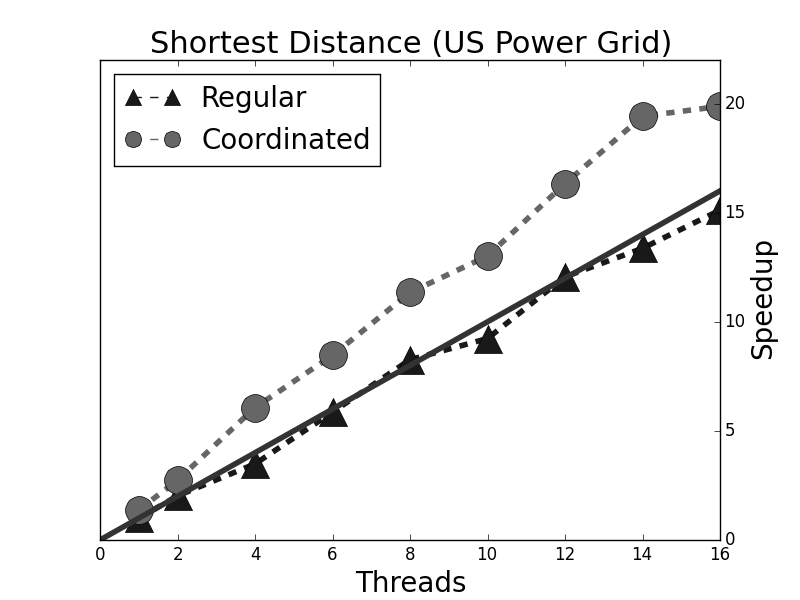
\includegraphics[width=5cm]{results/shortest-uspowergrid.png}}
   \end{center}
   \scap{results:sssp_uspowergrid}{Results for SSSP run on the 
   US power grid network.  On the left we show the number of facts
   derived for the regular \textbf{R} and coordinated
   version \textbf{C} using a variable number of threads \textbf{\#
   T}. On the right, we show the scalability of the regular and
   coordinated version. The speedup values are computed using the
   execution time for 1 thread.}
\vspace*{-3ex plus 0pt minus 1ex}
\end{topfig}


\subsection{MiniMax}

The MiniMax algorithm is a decision rule algorithm for minimizing the
possible loss for a worst case (maximum loss) scenario in a zero sum
game for 2 (or more) players that play in
turns~\cite{Edwards54}.

The algorithm builds a game tree, where each tree node represents a
game state and the children represent the possible game moves that can
be made by either player 1 or player 2.  An evaluation function is
used to compute the score of the board for each leaf of the tree. A
node is a leaf when the game state can no longer be expanded. Finally,
the algorithm recursively minimizes or maximizes the scores of each
node.  To select the best move for player 1, the algorithm picks the
move maximized at the root node.

In CLM, the program starts with a root node (with the initial game state)
that is expanded with the available moves at each level. The graph of the
program is dynamic since nodes are created and then deleted once they are no
longer needed. The latter happens when the
leaf scores are computed or when a node fully minimizes or maximizes the
children scores. When the program ends, only the root node has facts in its
database.

The code in Fig.~\ref{minimax:check-end} deals with the tree expansion process.
The first three rules (lines 1-10) deal
with the case where no children nodes are created and the last three rules
(12-29) deal with the cases that create new nodes. In particular, the two
rules in lines 12-26 generate new nodes using the
\mytt{exists} language construct, which creates a child node 
\mytt{B}. We link \mytt{B} with its parent (\mytt{parent(B, A)})
and kick start the expansion of that node \mytt{B} by adding a \mytt{play}
fact.

As noted in \sectref{sec:fifo}, the default scheduler is
breadth-first, which in this case leads to a complete expansion of the
tree before computing the scores at the leaves.  This results in using
$\mathcal{O}(n)$ memory, where $n$ is the number of nodes in the tree.

\begin{topfig}
\scriptsize\begin{Verbatim}[numbers=left,commandchars=\\\{\}]
expand(A, Board, [], 0, P, \underline{Depth})
  -o leaf(A, Board).

expand(A, Board, [], N, P, \underline{Depth}),
N > 0, P = player1
  -o maximize(A, N, -00, 0).

expand(A, Board, [], N, P, \underline{Depth}),
N > 0, P = player2
  -o minimize(A, N, +00, 0).

expand(A, Board, [0 | Xs], N, P, \underline{Depth}),
Depth >= 5
  -o exists B. (\underline{set-static(B)},
       \underline{set-default-priority(B, float(Depth + 1))},
       play(B, Board ++ [P | Xs], next(P), \underline{Depth + 1}),
       expand(A, Board ++ [0], Xs, N + 1, P, \underline{Depth}),
       parent(B, A)).

expand(A, Board, [0 | Xs], N, P, \underline{Depth}),
Depth < 5
  -o exists B. (
       \underline{set-default-priority(B, float(Depth + 1))},
       play(B, Board ++ [P | Xs], next(P), \underline{Depth + 1}),
       expand(A, Board ++ [0], Xs, N + 1, P, \underline{Depth}),
       parent(B, A)).

expand(A, Board, [C | Xs], N, P, \underline{Depth}) C <> 0
  -o expand(A, Board ++ [C], Xs, N, P, \underline{Depth}).
\end{Verbatim}
\scap{minimax:check-end}{MiniMax: checking if the game has ended and expanding the tree}
\vspace*{-2ex}
\end{topfig}
\normalsize

With coordination, we set the priority of a node to be its depth (lines 15 and
23) so that the tree is expanded in a depth-first fashion,
leading to a memory complexity of $\mathcal{O}(d t)$, where $d$
is the depth of the tree and $t$ is the number of threads.
Since threads prioritize deeper nodes, the scores of the first leaves are immediately
computed and then sent to the parent node. At this point, the leaves are deleted
and reused for other nodes in the tree, resulting in minimal memory usage.

\iffalse
As an example,
consider a system with 2 threads, $T_1$ and $T_2$, where $T_1$ first expands the root
node and then the first child. Since $T_2$ is idle, it steals half of the root's
children nodes and starts expanding one of the nodes in a depth-first fashion.
\fi

\iffalse
\begin{topfig}
   \begin{center}
      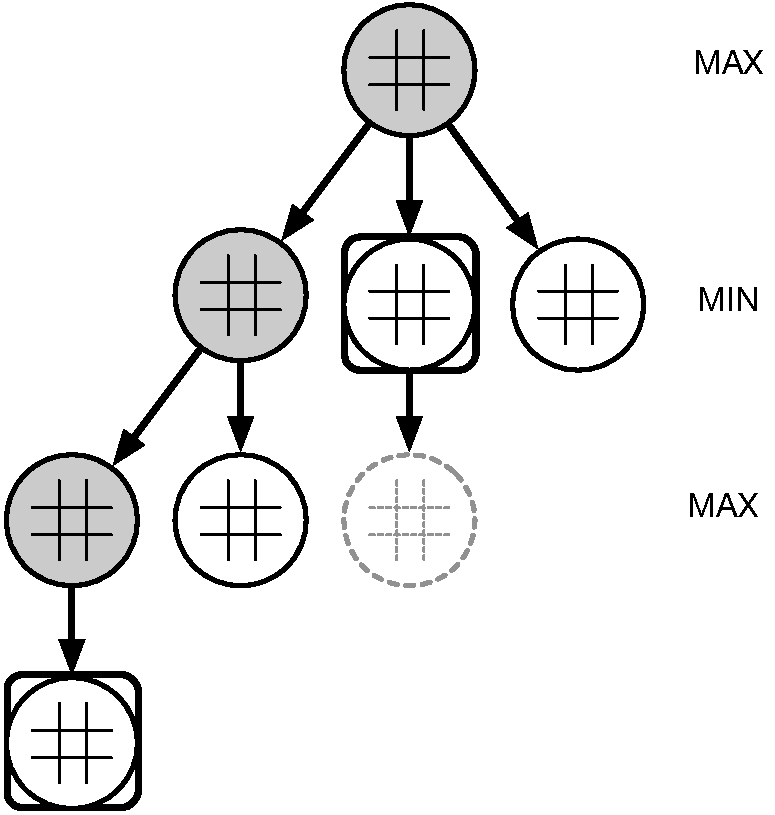
\includegraphics[width=4.5cm]{figures/minimax_tree}
   \end{center}
   \scap{fig:minimax}{Expanding the MiniMax tree using coordination. By prioritizing
      deeper nodes, threads are forced to expand the tree using a depth-first
      approach, which is superior since there is no need to expand the whole
      tree before computing the node scores.}
\end{topfig}
\fi

We also take advantage of memory locality by using \mytt{set-static} (line
14), so that nodes after a certain level are not stolen by other threads. While
this is not critical for performance in shared memory systems where node
stealing is fairly efficient, we expect that such coordination to be critical in
distributed systems.

\begin{topfig}
\vspace*{-3ex}
   \begin{center}
      \subfloat[]{\footnotesize\begin{tabular}[b]{ | c | c | c |}
         \hline                       
         \textbf{\# T} & \textbf{R} & \textbf{C} \\ \hline \hline
         1 & 11.80GB & 0.50MB \\ \hline
         2 & 12.19GB & 1.45MB \\ \hline
         4 & 13.82GB & 2.35MB \\ \hline
         8 & 14.87GB & 4.36MB \\ \hline
         16 & 13.79GB & 8.1MB \\ \hline
         \end{tabular}
         \normalsize
      }
      \subfloat[]{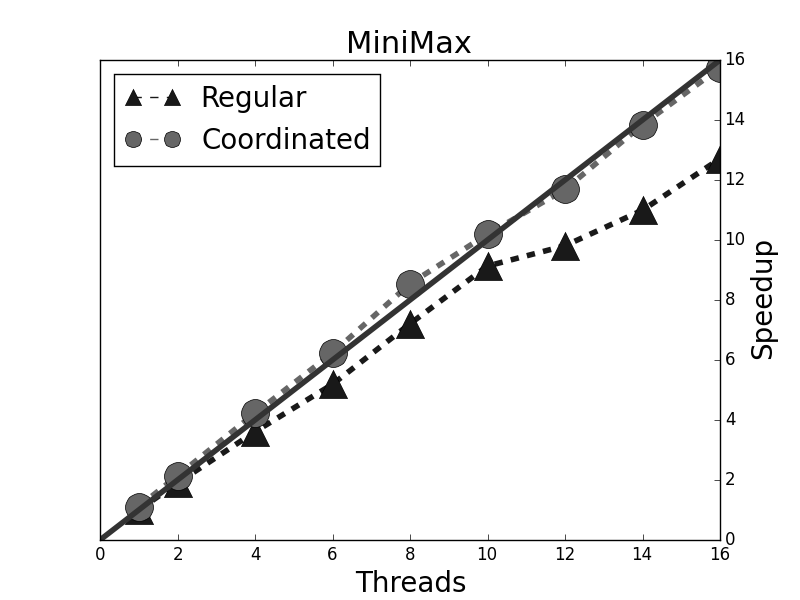
\includegraphics[width=4.5cm]{results/min-max-tictactoe.png}}
   \end{center}
   \scap{results:memory_minmax}{Memory usage and scalability of the regular and coordinated versions
      of MiniMax.}
\vspace*{-2ex}
\end{topfig}

In Fig.~\ref{results:memory_minmax} we compare the memory usage and scalability
of the coordinated MiniMax against the regular MiniMax. The coordinated version
uses significantly less memory (at most 8MB for 16 threads) than the regular
version (almost 14GB). Note that as the number of threads goes
up, memory usage also goes up. This is an artifact of our parallel memory
allocator that allocates large chunks of memory beforehand.
In terms of scalability, our experimental results show a 14-fold speedup for the
coordinated version against a 12-fold for the regular version when using 16
threads. When comparing the two versions directly, there is a 20\% run time
reduction when using 16 threads in the coordinated version.


\subsection{Heat Transfer}

In the Heat Transfer algorithm~(HT), we have a graph where heat values are
exchanged between nodes. The goal of the program is to exchange heat between
nodes. The program stops when the new heat values of every node are
$\delta = |H_i - H_{i-1}| \le \epsilon$. The algorithm works
asynchronously since heat values can be updated by using new partial information
coming from neighbor nodes. This increases parallelism since nodes do not need
to synchronize between iterations.

Fig.~\ref{code:ht} shows the HT rules that send new heat values to
neighbor nodes. In the first rule we added \texttt{add-priority} to increase the priority of the neighbor
nodes if the current node has a large $\delta$. The idea is to prioritize the
computation of heat values of nodes (using \texttt{update}) that have a neighbor
that changed significantly. Multiple \texttt{add-priority} facts will
increase the priority of a node so that nodes with multiple large deltas will
have more priority.

\begin{figure}[h!]
\scriptsize\begin{Verbatim}[numbers=left,commandchars=\\\[\]]
new-heat(A, New, Old),
Delta = fabs(New - Old),
Delta > epsilon
   -o {B, W | !edge(A, B, W) |
         new-neighbor-heat(B, A, New),
         update(B), \underline[add-priority(B, Delta)]}.

new-heat(A, New, Old)
fabs(New - Old) <= epsilon
   -o {B, W | !edge(A, B, W) |
         new-neighbor-heat(B, A, New)}.
\end{Verbatim}
  \caption{Coordination code for the Heat Transfer program. We updated the first rule
     to increase the priority of neighbor nodes.  The code logic remains exactly
     the same as before, however bigger changes in heat values are now
     propagated faster.}
  \label{code:ht}
\end{figure}
\normalsize

Fig.~\ref{results:ht} presents the scalability results for the uncoordinated
and coordinated version. The dataset used is a square grid with an inner square
with high heat nodes. With 1 thread, there's a 33\% reduction in run time, while
for 16 threads, there's a 18\% reduction.

To further improve locality, we split the second rule to
not send small $\delta$ values if the target node is in another
thread. XXX talk about results

\begin{figure}[h!]
\scriptsize\begin{Verbatim}[numbers=left,commandchars=\\\[\]]
new-heat(A, New, Old)
fabs(New - Old) <= epsilon
\underline[cpu-id(A, B, C)],
\underline[cpu-id(A, A, C)]
   -o {B, W | !edge(A, B, W) |
         new-neighbor-heat(B, A, New)}.

new-heat(A, New, Old)
fabs(New - Old) <= epsilon,
\underline[cpu-id(A, B, C1)],
\underline[cpu-id(A, A, C2)],
\underline[C1 <> C2]
   -o 1. // nothing is derived
\end{Verbatim}
  \caption{To improve locality, we added a third rule to not send small $\delta$
     values if the neighbor is in another thread.}
  \label{code:ht_better}
\end{figure}
\normalsize

\begin{figure}[ht!]
   \begin{center}
      \subfloat[]{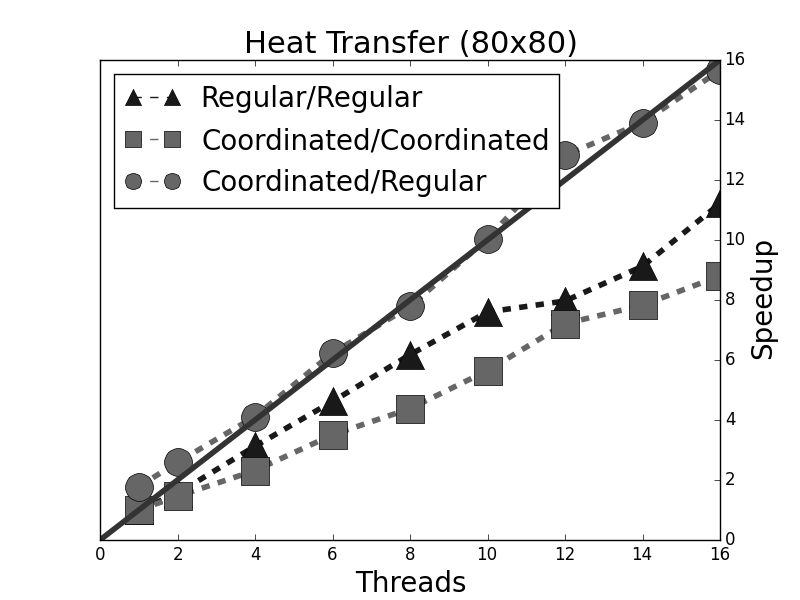
\includegraphics[width=5cm]{results/new-heat-transfer-80}}
   \end{center}
   \caption{Experimental results for the HT program. The coordinated version
      is, on average, 30\% faster than the regular version although it has a
      slightly worse scalability due to a reduction in work available.}
   \label{results:ht}
\end{figure}


\subsection{Splash Belief Propagation}

Randomized and approximation algorithms can obtain significant benefits from
coordination directives because their inherent non-determinism can be harnessed
to evaluate rules in different orders.
An example of such program is Loopy Belief Propagation.
Loopy Belief Propagation~\cite{Murphy99loopybelief} (LBP) is an approximate inference algorithm
used in graphical models with cycles. In its essence, LBP is a sum-product message passing algorithm
where nodes exchange messages with their immediate neighbors and apply some computations to the messages
received.

LBP is an algorithm that maps very well to the graph based model of CLM. In its
original form, the belief values of nodes are computed by synchronous iterations.
LBP offers more concurrency when belief values are computed asynchronously
leading to faster convergence. For this, every node keeps track of all messages
sent/received and recomputes the belief using partial information from neighbor
nodes. It is then possible to prioritize the computation of beliefs when a
neighbor's belief changes significantly.

The asynchronous approach proves to be a nice improvement over the synchronous
version. Still, it is possible to do even better. Gonzalez et
al~\cite{Gonzalez+al:aistats09paraml} developed an optimal algorithm to compute
this algorithm by first building a tree and then updating the beliefs of each
node twice, first from the leaves to the root and then from the root to the
leaves. The root of this tree is the node with the highest priority (based on
belief) while the other nodes in the tree must have a non-zero priority.
Note that the priorities are updated whenever a neighbor updates their belief.
These \emph{splash trees} are built iteratively until we reach convergence.
%In Fig.~\ref{splash_bp} we represent two threads creating two different splash trees.

\iffalse
\begin{topfig}
   \begin{center}
      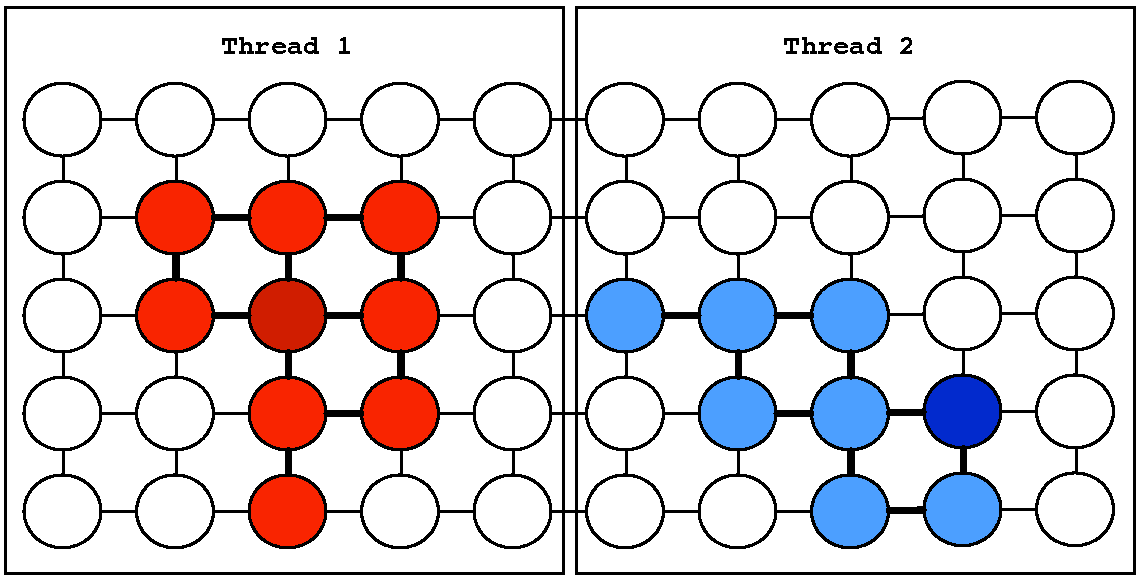
\includegraphics[width=6.5cm]{figures/splash_bp}
   \end{center}
   \scap{splash_bp}{Creating splash trees for belief propagation. Each threads picks the
   highest priority node and creates a tree from that node. The belief values
   are updated in two phases: first from the leaves to the root and then from
   the root to the leaves.}
\end{topfig}
\fi

The code for Splash Belief Propagation~(SBP) in Fig.~\ref{code:sbp} presents the
coordination code for LBP.  Please note that we just appended the code in
Fig.~\ref{code:sbp} to a working but unoptimized version of the algorithm, every
other rule remains the same. We add new rules that coordinate
the creation and execution of the splash trees:

\begin{tightdescription}
   \item[Tree building]: Each node has a \texttt{inactive} fact that is used to
   start the tree building process. When the highest priority node is picked, a
   \texttt{tree} is created that will navigate through the tree. In lines 15-21,
   we use an \emph{aggregate}~\cite{cruz-iclp14} to gather all the neighbor
   nodes that have a positive priority (due to a new belief update) and are in the
   same thread. Nodes are collected into list \texttt{L} (line 21) and
   appended to list \texttt{Next}.
   
   \item[First phase]: In the
   third rule (lines 11-12), when the number of nodes of the tree reaches a
   certain limit, a \texttt{first-phase} is generated to update the beliefs of
   all nodes in the tree, starting from the leaves and ending at the root As the
   nodes are updated, an \texttt{update} fact is derived to update the belief
   values (line 35).

   \item[Second phase]: In the second phase, the computation of beliefs is
   performed from the root to the leaves and the belief values are updated a
   second time (line 42).
\end{tightdescription}

The \texttt{set-static} and \texttt{set-cpu} action facts are used in
line 2 to (1) force nodes to stay in the thread and (2) 
partition nodes as a grid of threads. This sets up well defined areas
of nodes for threads to build splash trees on.

\begin{topfig}
\scriptsize\begin{Verbatim}[numbers=left,commandchars=*\{\}]
!coord(A, X, Y), start(A)
   -o *underline{set-static(A), set-cpu(A, grid(X, Y))}.

// TREE BUILDING
// expand tree by adding neighbor nodes
inactive(A), tree(A, All, Next) -o expand-tree(A, All, Next).
// start tree since we do not have one
inactive(A), *underline{@priority(A, A, P)}, P > 0.0
   -o expand-tree(A, [A], [A]).
// end tree building
expand-tree(A, All, Next), length(All) >= maxnodes
   -o first-phase(A, All, reverse(All)).
// expand tree
expand-tree(A, All, [A | Next]), length([A | Next]) < maxnodes
   -o [collect => L | Side | !edge(A, L, Side),
         0 = count(All, L), // L is not in All
         0 = count(Next, L), // L is not in Next
         *underline{@priority(A, L, P), P > 0.0,}
         *underline{@cpu-id(A, L, Id1)},
         *underline{@cpu-id(A, A, Id2), Id1 = Id2} |
         send-tree(A, All, Next ++ L)].

send-tree(A, All, [])
   -o first-phase(A, All, reverse(All)).
send-tree(A, All, [B | Next])
   -o *underline{schedule-next(B)},
      tree(B, All ++ [B], [B | Next]).

// FIRST PHASE
first-phase(A, [A], [A]) -o second-phase(A, [], A).
first-phase(A, [A, B | Next], [A])
   -o update(A), *underline{schedule-next(B)},
      second-phase(B, [B | Next], A).
first-phase(A, All, [A, B | Next])
   -o update(A), *underline{schedule-next(B)},
      first-phase(B, All, [B | Next]).

// SECOND PHASE
second-phase(A, [], _)
   -o *underline{set-priority(A, 0.0)}, inactive(A), update(A).
second-phase(A, [A], Back)
   -o update(A), inactive(Back),
      inactive(A), *underline{set-priority(A, 0.0)}.
second-phase(A, [A, B | Next], Back)
   -o update(A), inactive(Back), *underline{schedule-next(B)},
      second-phase(B, [B | Next], A).
\end{Verbatim}
  \scap{code:sbp}{Coordination code for the Splash Belief Propagation program. 
%CLM needs 50 lines of rules to implement splash trees, while GraphLab needs a total of 350 lines of C++ to implement the same functionality.
  Note
     that when a linear fact is prefixed by \texttt{@}, it indicates that the
     fact is going to be re-derived.}
\end{topfig}
\normalsize

\begin{dblfig}
   \begin{center}
      \subfloat[]{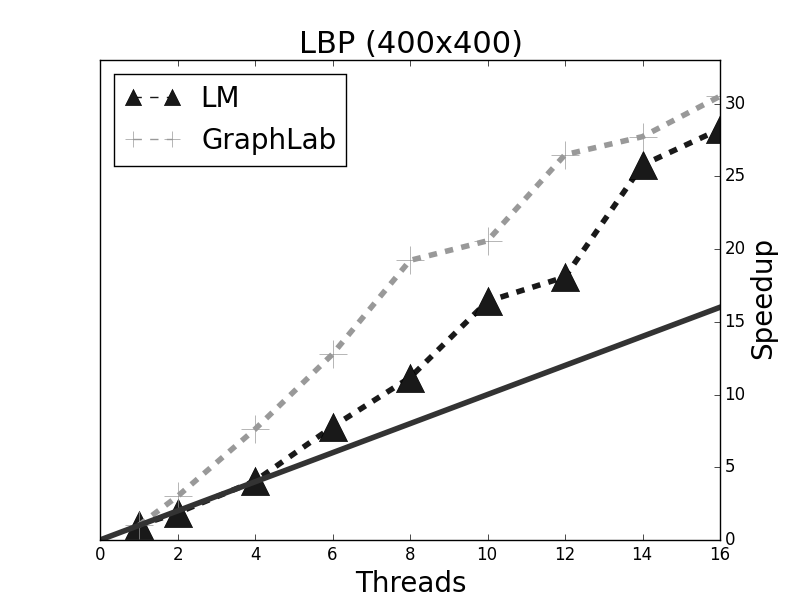
\includegraphics[width=5.5cm]{results/system_belief-propagation-400.png}}
      \subfloat[]{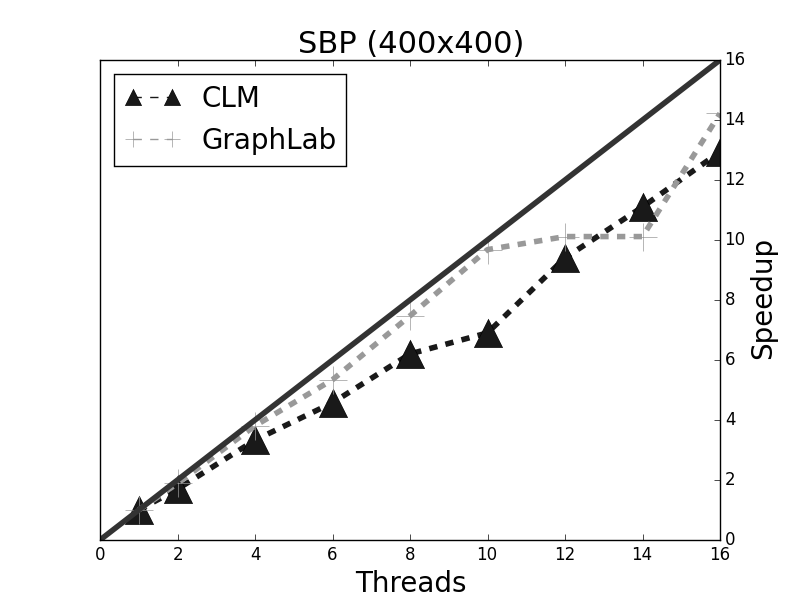
\includegraphics[width=5.5cm]{results/system_splash-bp-400.png}}
      \subfloat[]{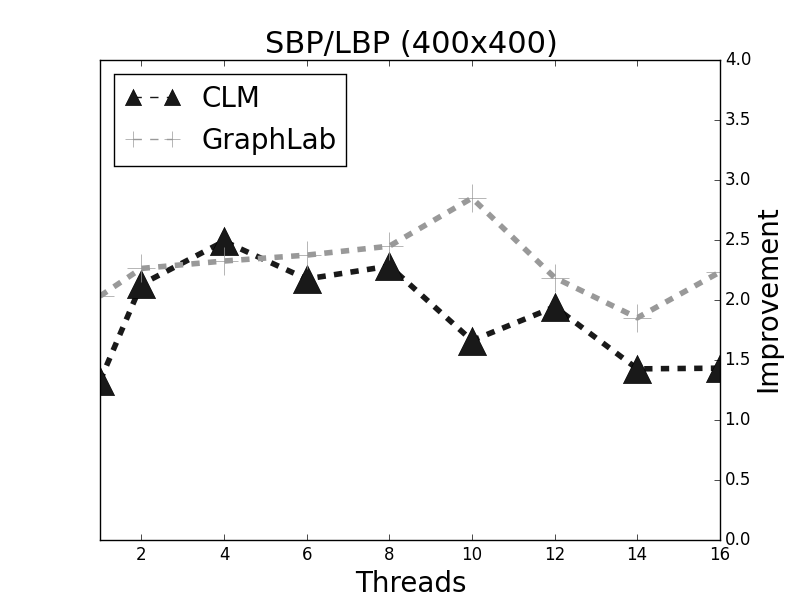
\includegraphics[width=5.5cm]{results/system_improve_belief-propagation-400.png}}
   \end{center}
   \scap{results:splash_bp}{Experimental results for LBP and SBP. (a) shows the
      scalability of LBP for both CLM and GraphLab and (b) shows the
      scalability of SBP. (c) presents the
      improvements seen in SBP against LBP, where SBP runs, on average, 1.5 to 2.5
      times faster than LBP.}
\end{dblfig}

In this program, coordination assumes a far more important role than
we have seen before. Coordination rules fully drive the behavior of
the algorithm and although the final result of the algorithm is
statistically identical to the original algorithm, SBP works very
differently than LBP.  SBP is also implemented in
GraphLab~\cite{GraphLab2010}, a C++ framework for writing machine
algorithms.  GraphLab provides the splash scheduler as part its the
framework. It is 350 lines of C++ code.  With our coordination facts,
it is possible to create the necessary scheduling with only 12 rules.

We measured the behavior of LBP and SBP for both CLM and GraphLab.
Fig.~\ref{results:splash_bp} shows that both systems have very similar behavior
when using a variable number of threads.  The differences in performance between
GraphLab and CLM comes mainly because GraphLab performs in-place updates of
neighbor belief values, while CLM compiler and runtime system performs naive
manipulation of facts by deriving rules. The in-place update could be generated
by the compiler using smarter compilation strategies.


\subsection{N Queens}


\section{Conclusions}
We think that our particular approach is applicable in distributed systems as we
have seen. Explore functional programming and coordination?


\section{Acknowledgements}

\input{ack}

\bibliographystyle{abbrvnat}
\bibliography{refs}

\end{document}
